% coding:utf-8

%----------------------------------------
%FOSADSVB, a LaTeX-Code for a summary of digital signal processing
%Copyright (C) 2015, Mario Felder & Michi Fallegger

%This program is free software; you can redistribute it and/or
%modify it under the terms of the GNU General Public License
%as published by the Free Software Foundation; either version 2
%of the License, or (at your option) any later version.

%This program is distributed in the hope that it will be useful,
%but WITHOUT ANY WARRANTY; without even the implied warranty of
%MERCHANTABILITY or FITNESS FOR A PARTICULAR PURPOSE.  See the
%GNU General Public License for more details.
%----------------------------------------

\chapter{Analog-Digital \& Digital-Analog Wandlung}
\section{Schritte der A/D- und D/A-Wandlung}
\textbf{Sample:} Kontinuierliche Signalwerte werden mit der Samplefrequenz
$f_S$ aufgezeichnet. Dies erzeugt eine Sequenz von diskreten Signalwerten.\\
\textbf{Quantize:} Die diskreten Signalwerte werden einer bestimmten
Anzahl Quantisierungsleveln zugeordnet.\\
\textbf{Code:} Die quantisierten Abtastwerte können verwendet werden,
um die erhaltene Pulsfolge zu modulieren (Pulse Code Modulation PCM). Meistens
wird die Signalverarbeitung direkt mit den quantisierten Abtastwerten vorgenommen,
so dass diese ohne Modulation gespeichert werden. Dazu wird die Repräsentierung
der Quantisierungsleveln benötigt.\\\\
Die Digital-Analog Wandlung enthält folgende Schritte:\\
\textbf{Decode:} Die digitalen Werte werden in einer für die Digital-Analog
Wandlung repräsentativer Form benötigt.\\
\textbf{Hold:} Das diskrete Signal muss über die Sampleperiode $T_S$ konstant
gehalten werden, ein Treppen-ähnlicher Output entsteht.\\
\textbf{Interpolate:} Das kontinuierliche Treppensignal wird durch Mittelwerte
von Tiefpass-Filtern geglättet.

\begin{center}
	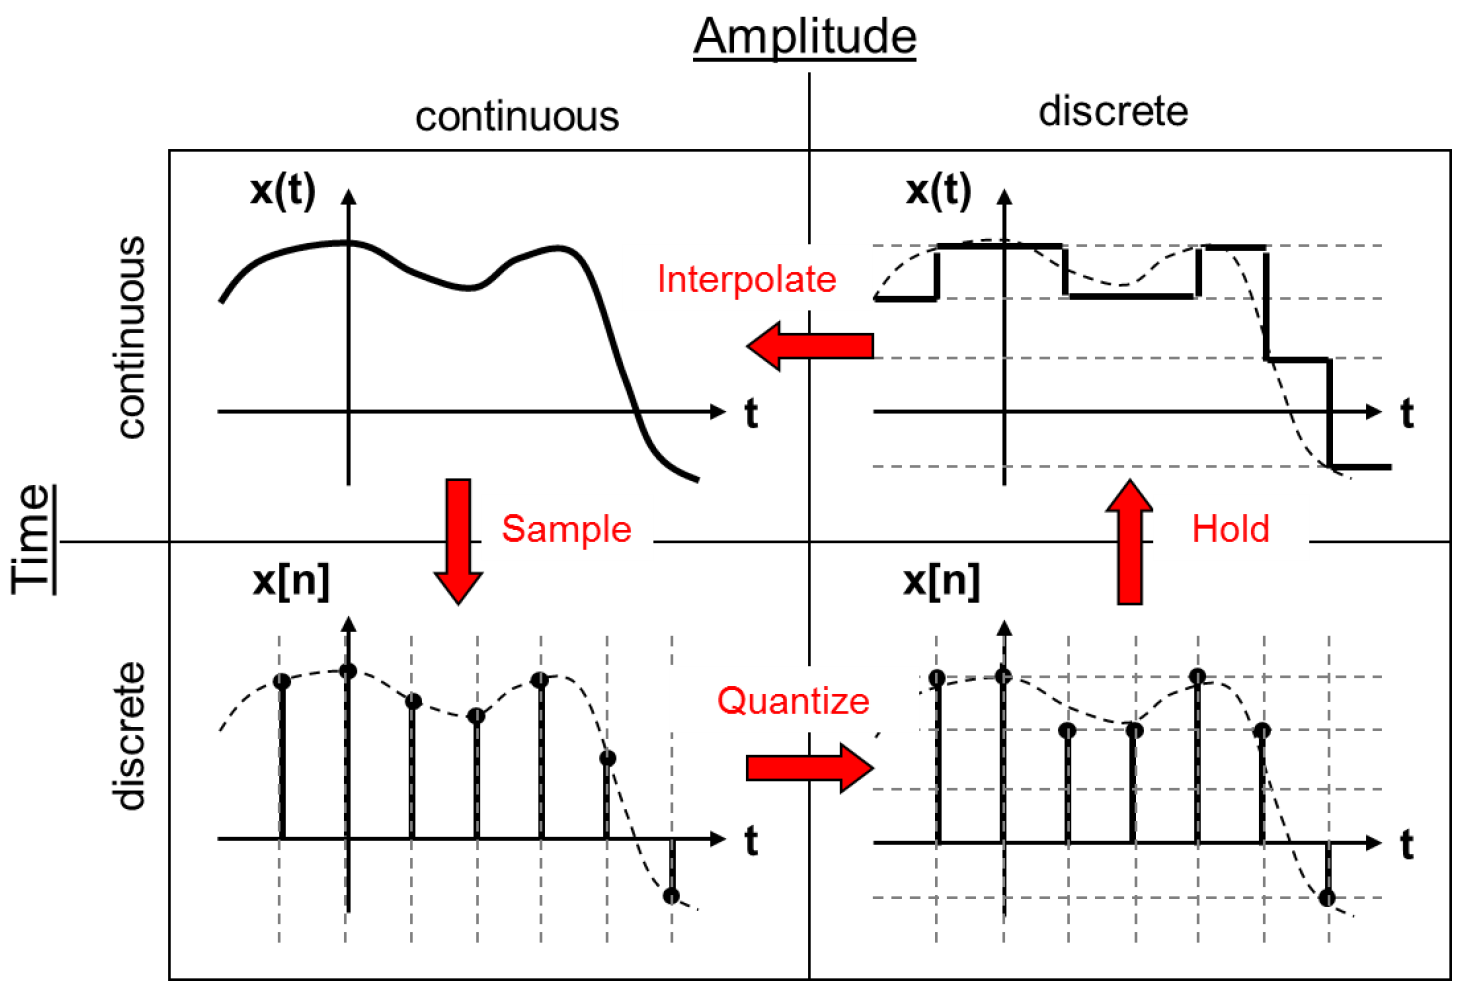
\includegraphics[scale=.85]{../fig/ad_da}
\end{center}
\section{Digitale Signalprozessoren (DSP)}
Ein DSP prozessiert das digitale Signal nach einem vorgegebenen Algorithmus in SW-Form. Übliche Anwendungen:
\begin{itemize}[itemsep=-5pt,topsep=3pt]
	\item \textbf{Signalgenerierung:} Harmonische \& Random-Signale, wichtig im Bereich Mess- und Kommunikationstechnik.
	\item \textbf{Signalanalyse:} Analyse im Zeit- oder Frequenzbereich
	\item \textbf{Signalkomposition:} Zusammenführen, in der Zeitdomaine üblicherweise mittels Korrelationstechnik. In der Kommunikationstechnik wird im Frequenzbereich korreliert, um eine Modulation des Signals zu erreichen. 
\end{itemize}
Vorteile:
\begin{itemize}[itemsep=-5pt,topsep=3pt]
	\item \textbf{Programmierbarkeit:} Selbe HW kann für Anwendung verwendet und einfach neu programmiert werden.
	\item \textbf{Parametrisierbarkeit:} Parameter können ohne Hardware-Anpassungen geändert werden, teils sogar automatisch.
	\item \textbf{Wiederholbarkeit:} Resultate können exakt reproduziert werden, keine Alterungserscheinungen o.ä.
\end{itemize}
Nachteile:
\begin{itemize}[itemsep=-5pt,topsep=3pt]
	\item Zusätzlicher Aufwand für AD und DA-Wandlung.
	\item (Noch) keine Prozessierung von HF-Signalen möglich.
	\item Potentielle EMV-Probleme mit analoger HW.
\end{itemize}
%===============================================================================
\section{Abtasten und Aliasing}
\subsection{Abtasten von Tiefpass-Signalen}
Mathematisch wird die Abtastung des Signals $x(t)$ durch eine Multiplikation
mit Dirac-Impulsen der Periode $T_S$ dargestellt. Es entsteht ein Zug aus gewichteten Dirac-Impulsen. 
\[ x_s(t) = \sum_{n=-\infty}^{\infty} x(t) \cdot \delta(t-nT_S) \]
Das Frequenzspektrum des abgetasteten Signals ist:
\[ X_S(f) = \frac{1}{T_S} \sum_{k=-\infty}^{\infty} X(f-kf_S) \]

\begin{center}
	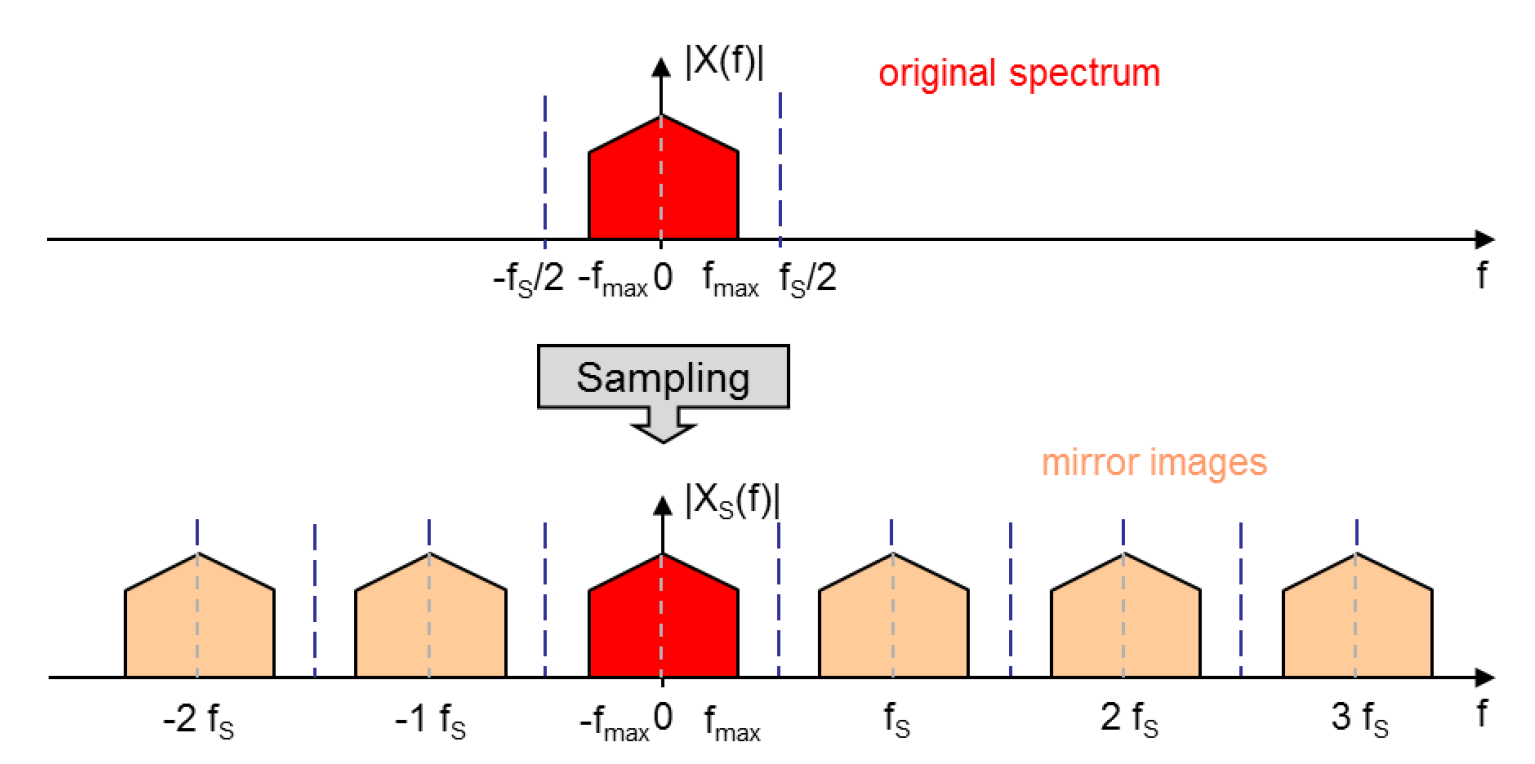
\includegraphics[scale=0.9]{../fig/frequenz_spectrum}
\end{center}
Um das Signal rekonstruieren zu können, müssen die Spiegelfrequenzen von $X(f)$
mit einem Tiefpassfilter unterdrückt werden. Das geht nur, wenn die grösste
Frequenz $f_{max}$ des Signals kleiner als die halbe Abtastfrequenz $f_S/2$ ist, sich die "'mirror images"' also nicht überlappen.
Aus dem \textbf{Nyquist-Kriterium} oder \textbf{Abtasttheorem} folgt:
\[ f_S > 2 \cdot f_{max} \]

%===============================================================================
\subsection{Aliasing \& Gegenmassnahme}
Aliasing entsteht, wenn das Abtasttheorem verletzt wird. Die Frequenzanteile
über $f_S/2$ werden in das Basisband gespiegelt und überlagern mit den 
gewünschten Frequenzen. Das analoge Signal kann nicht rekonstruiert werden.\\
Dem kann mit einer Tiefpassfilterung \emph{vor} der Abtastung entgegengewirkt werden. Ausserhalb des gewünschten Frequenzbandes $f_{desired}$ darf es hingegen zu Aliasing kommen. Es gelten die Filter-Spezifikationen:
\[ f_{pass} \geq f_{desired} \hspace{10mm} \mathrm{sowie} \hspace{10mm} f_{stop} \leq f_S - f_{desired} \]

\begin{minipage}{.475\textwidth}
	\begin{center}
		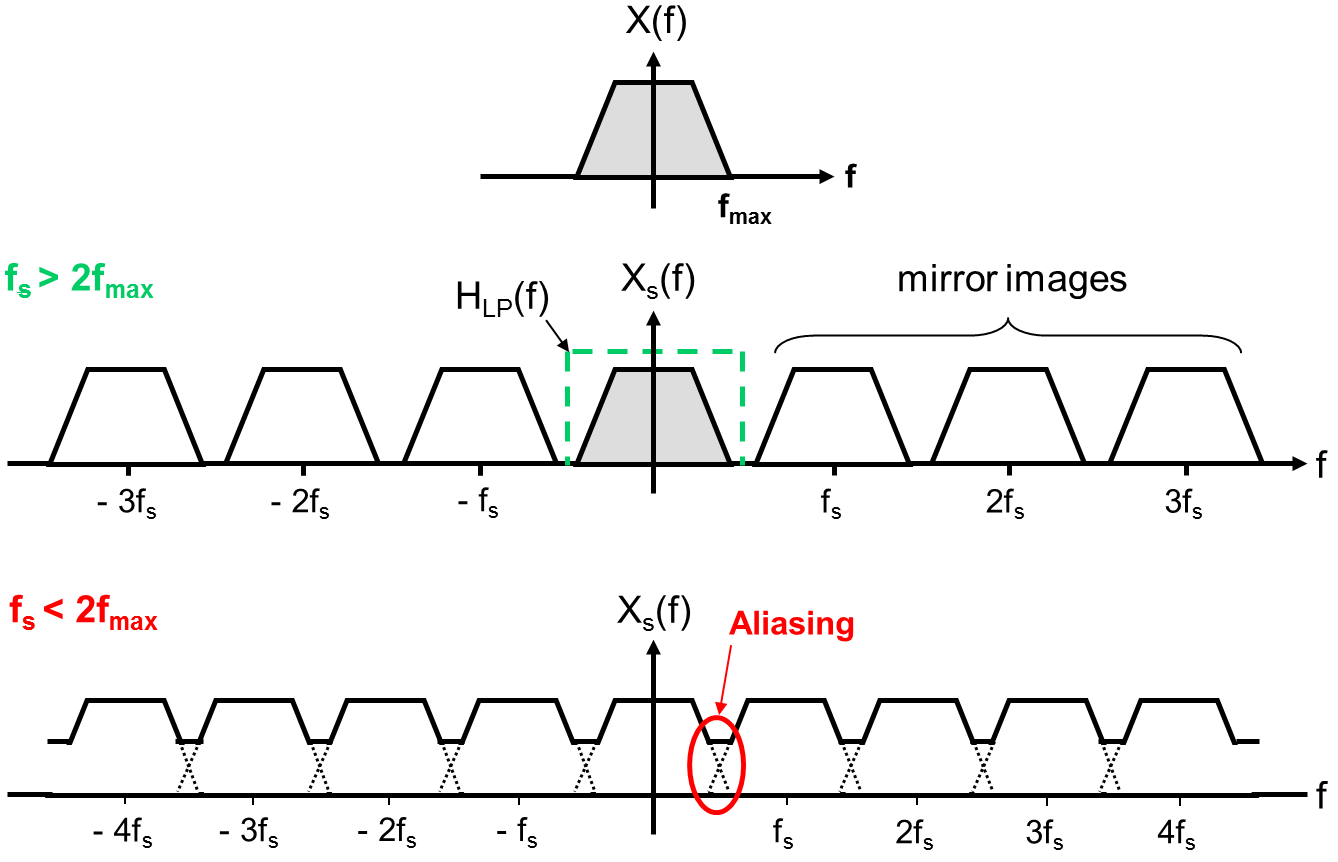
\includegraphics[width=\textwidth]{../fig/aliasing_frequency_domain}
	\end{center}
\end{minipage}
\begin{minipage}{.475\textwidth}
	\begin{center}
		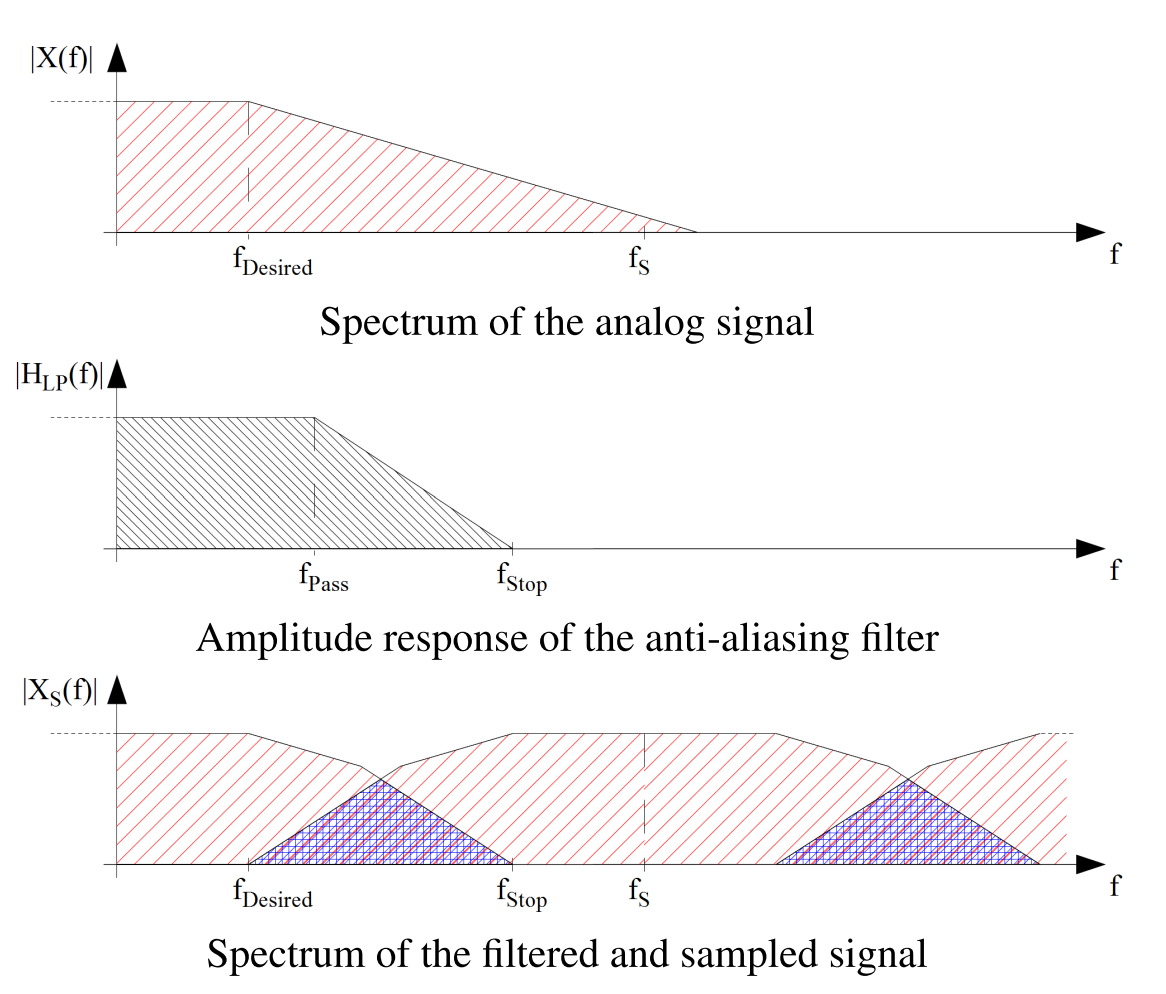
\includegraphics[width=\textwidth]{../fig/aliasing}
	\end{center}
\end{minipage}

%===============================================================================
\subsection{Abtasten von Bandpass-Signalen}
Um Bandpass-Signale zu sampeln, wird das Abtasttheorem angepasst (für $N\geq 1$), $f_S$ muss die Bedingung erfüllen:
\[ \frac{2\cdot f_{min}}{N} \geq f_S \geq \frac{2\cdot f_{max}}{N+1} \]
Beim Sampeln von Bandpass-Signalen wird der sonst unerwünschte Effekt des Aliasing ausgenützt. Für ungerade $N$ erscheint das originale Spektrum invertiert im Basisband.
Die originale Struktur des Spektrum wird zurückgewonnen durch Invertierung jedes zweiten Samples im Zeitbereich. Dies entspricht einer Frequenzverschiebung von der halben Abtastfrequenz $f_s$.
\[ \tilde{x}[n] = (-1)^n \cdot x[n] \]

\begin{minipage}{.475\textwidth}
	\begin{flushleft}
		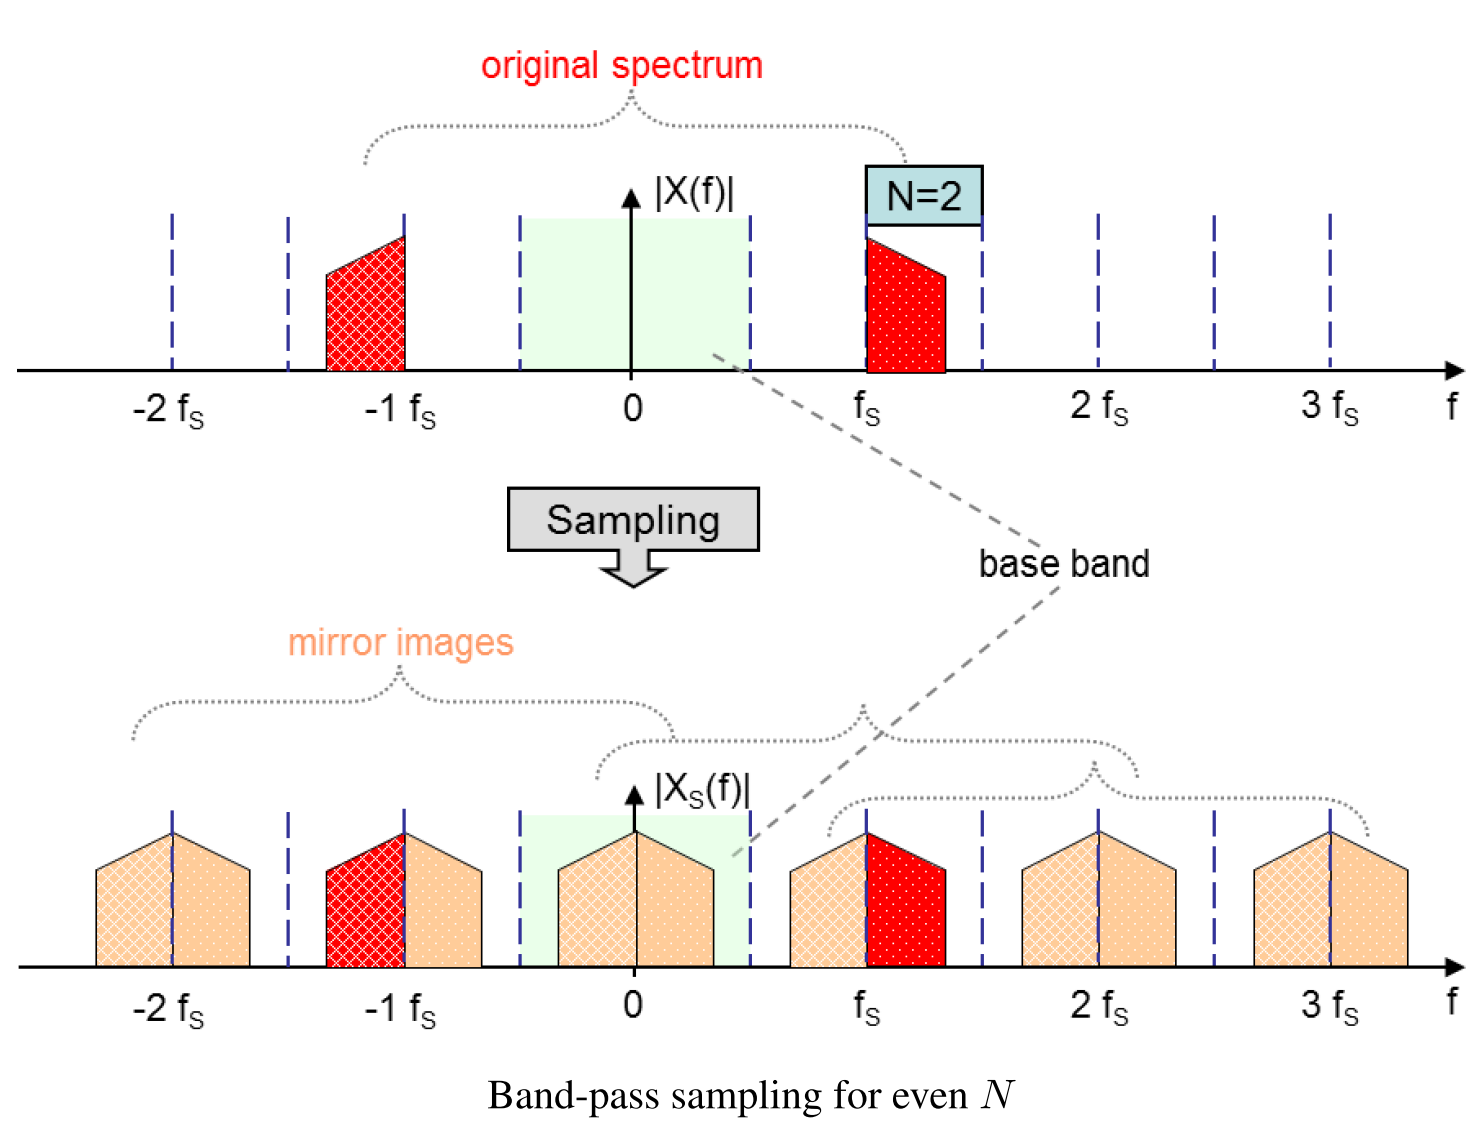
\includegraphics[width=\textwidth]{../fig/bandpass_even}
	\end{flushleft}
\end{minipage}
\begin{minipage}{.475\textwidth}
	\begin{flushleft}
		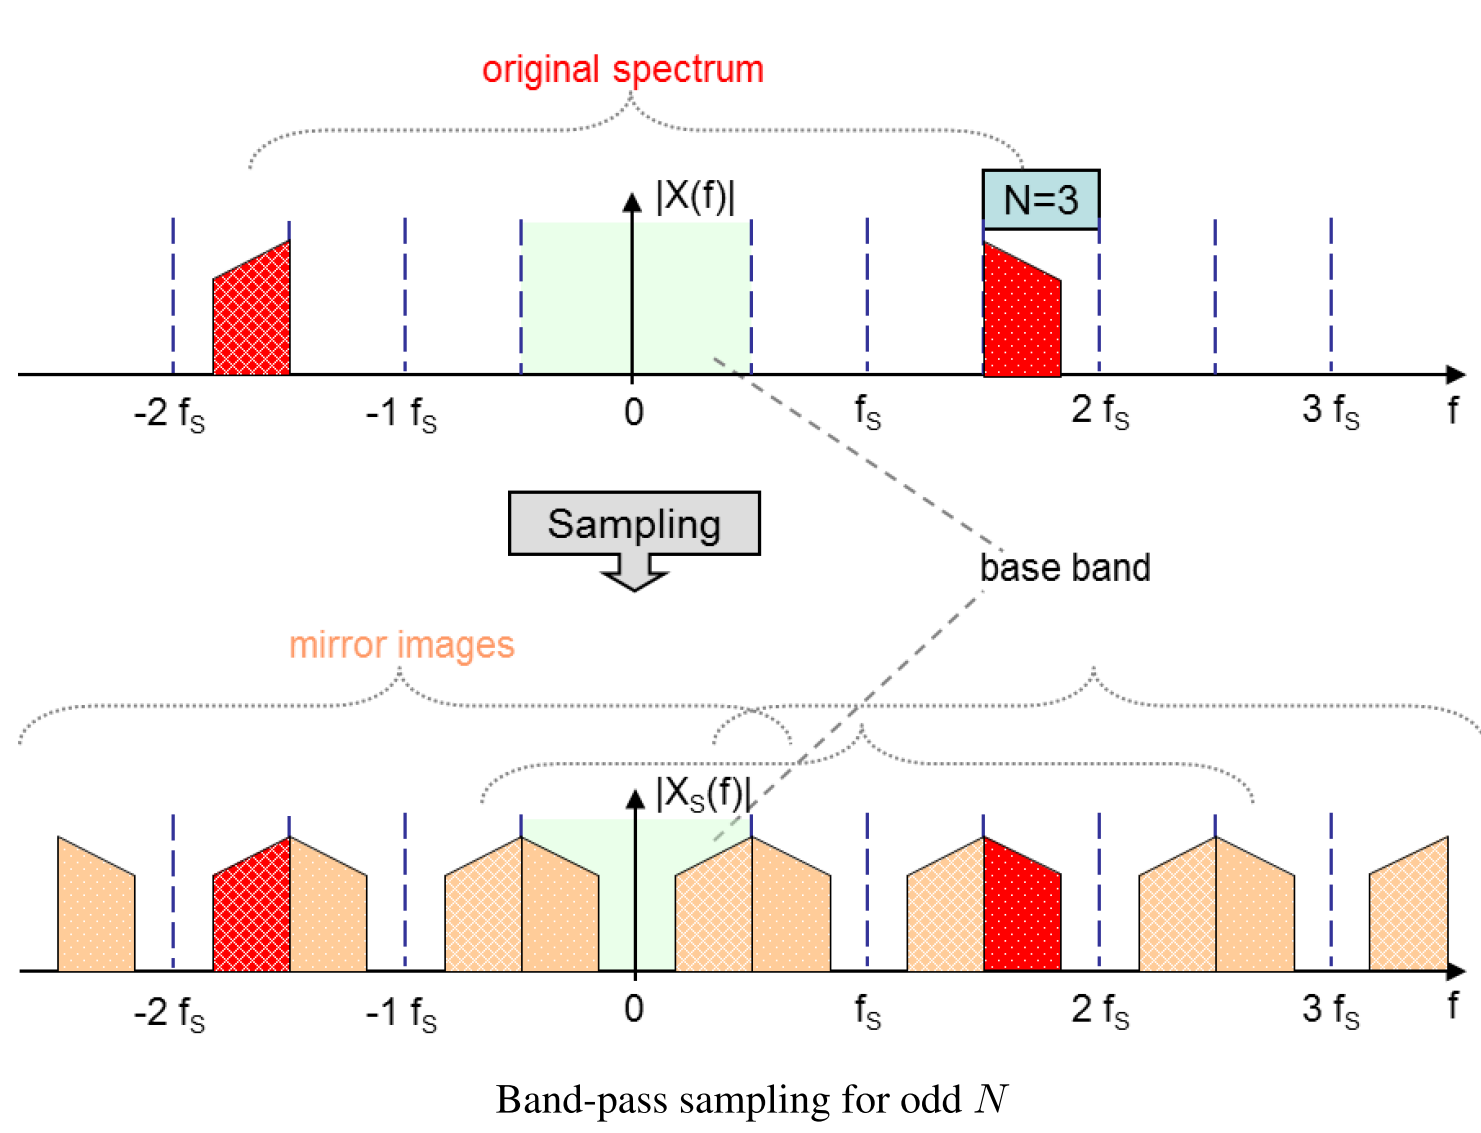
\includegraphics[width=\textwidth]{../fig/bandpass_odd}
	\end{flushleft}
\end{minipage}

%===============================================================================
\section{Quantisierung von Signalen}
\subsection{Uniforme Quantisierung}
Der Quantisierungsschritt (\textbf{quantization step}) $\Delta$ ist gegeben
durch die Auflösung mit $W$ Bits und der dynamischen Reichweite $R$ des
abgetasteten Signals $x[n]$:
\[ \Delta = \frac{R}{2^W} \]
Bei der uniformen Quantisierung ist die Schrittgrösse entlang der x- und y-Achse uniform (gleichmässig) verteilt. 
Es existieren zwei unterschiedliche Arten der Quantisierung: 
\begin{itemize}[noitemsep,topsep=3pt]
	\item Mid-tread quantizer: Entscheidungslevel bei $(\pm 0.5\Delta, \pm 1.5\Delta, \pm 2.5\Delta,...)$, 0-Level Output möglich
	\item Mid-rise quantizer: Entscheidungslevel bei $(\pm 0\Delta, \pm 1\Delta, \pm 2\Delta,...)$, einfachere Implementation in HW \& SW
\end{itemize}\vspace{11pt}
Durch das Abbilden eines amplitudenkontinuierlichen Signals auf eine endliche
Anzahl von Rekonstruktionsleveln können zweier Fehler entstehen:\\
\textbf{Clipping:} Werte von $x[n]$ ausserhalb des Bereichs $R$ werden mit
dem maximum bzw. minimum Rekonstruktionslevel dargestellt.\\\\
\textbf{Quantization error $\epsilon$:} Dieser Fehler tritt immer auf und
kann nicht verhindert werden. Die Grösse des Fehlers ist gegeben durch die
Qunatisierungsgrösse $\Delta$.\\
Für den mid-tread quantizer (runden zum nächsten Wert):
\[ -\Delta/2 < \epsilon \leq \Delta / 2 \]
Für den mid-rise quantizer (runden Richtung -$\infty$):
\[ -\Delta < \epsilon \leq 0 \]
\newpage 

%===============================================================================
\subsection{Quantisierungsrauschen}
Der Quantisierungsfehler zeigt sich als Rauschen überlagert zum quantisierten
Signal:
\[ \epsilon[n] = x_q[n] - x[n] \]
Die Leistung $P_\epsilon$ des Quantisierungsrauschens
(\textbf{quantization noise}) wird ausgedrückt mit:
\[ P_\epsilon = {\sigma_\epsilon}^2 = \int_{-\infty}^{\infty} (\epsilon - 
	{\sigma_\epsilon})^2 \cdot p(\epsilon) \di\epsilon = 
	\frac{\Delta^2}{12}\]
wobei $p(\epsilon)$ die Wahrscheinlichkeitsdichte ist. Angenommen die Werte
von $\epsilon[n]$ sind statistisch unkorreliert und uniform verteilt über den
Intervall $(-\Delta/2, \Delta/2]$, ist die Wahrscheinlichkeitsdichte für einen
mid-tread quantizer:
\[ p(\epsilon) = 1/\Delta \] 
Der Erwartungswert des Quantisierungsfehlers $\mu(\epsilon)$ ergibt somit:
\[ \mu(\epsilon) = \int_{-\infty}^{\infty} \epsilon \cdot p(\epsilon) 
	\di\epsilon = \left. \frac{1}{2\Delta}\epsilon^2
	\right|_{-\Delta/2}^{\Delta/2} = 0 \]
Das Modell zur Berechnung des Quantisierungsfehlers sowie die Fehlerverteilung 
bei einem mid-tread quantizer. 
\begin{center}
	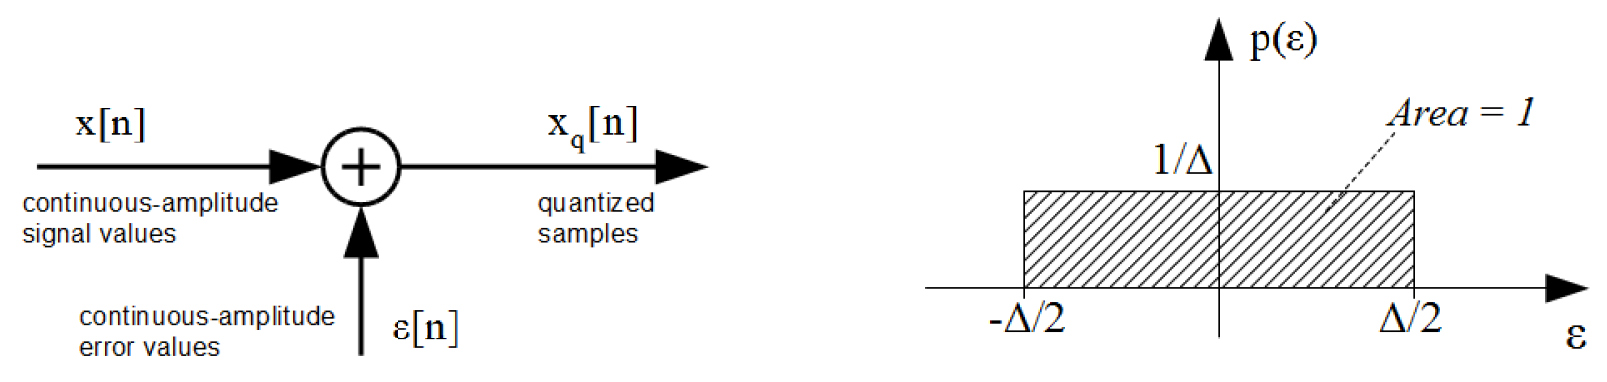
\includegraphics[width=.8\textwidth]{../fig/quantization_noise}
\end{center}
Für das Signal-Rausch-Verhältnis (SNR) gilt:
\[ SNR = \frac{P_x}{P_\epsilon} = 2^{2W} \cdot \frac{12 \cdot P_x}{R^2} \]
Durch Ausdrücken des SNR in dB ergibt sich:
\[\begin{aligned} SNR_{dB} &= 10 \cdot \left( \log_{10}2^{2W} +
	 \log_{10}\frac{12P_x}{R^2} \right)\\
	 &\approx 6W + 10 \cdot \log_{10}\frac{12P_x}{R^2} 
\end{aligned}\]
Bei einem harmonischen Inputsignal $x[n]$ ergibt sich folgendes SNR für
eine uniforme Quantisierung:
\[ SNR_{db} = 6W +1.76 \approx 6W \]
\textbf{Wichtige Faustformel:} Mit jedem zusätzlichen Bit und uniformer Quantisierung erhöht sich das SNR um 6 dB.
\newpage
\subsection{Logarithmische Quantisierung}
Eine Möglichkeit das mit der Quantisierung verbundene SNR zu verbessern, besteht darin, die Quantisierung auf die statischen Eigenschaften des Signales anzupassen. Dieser Ansatz ist besonders vielversprechend für
Signalklassen, die erheblich von einer gleichmäßigen Verteilung abweichen. 
Ein bekanntes Beispiel für eine solche Signalklasse sind menschliche Sprachsignale. Bei dieser Art von Signalen sind kleine Amplitudenwerte wahrscheinlicher als große Amplitudenwerte.
\begin{center}
	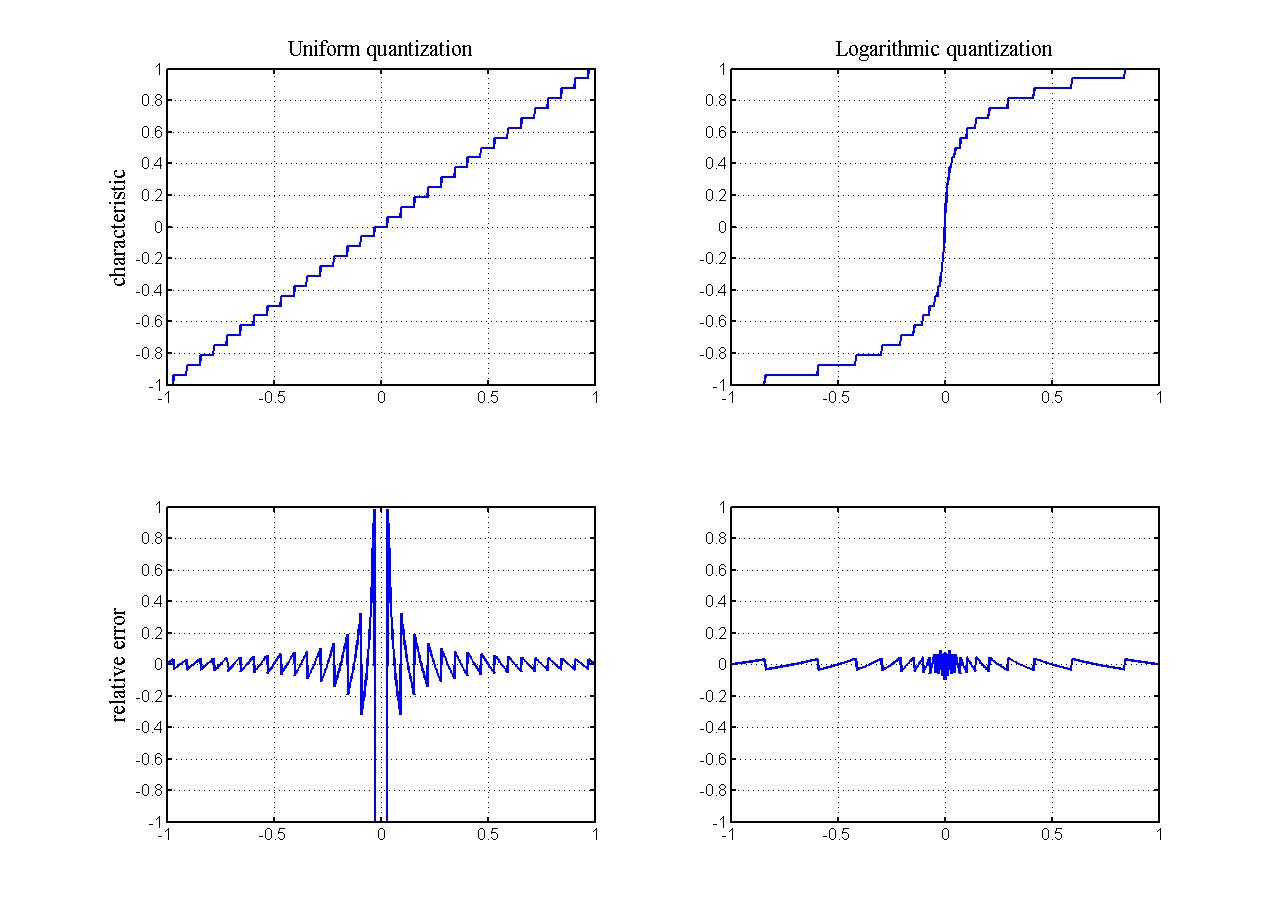
\includegraphics[width=.9\textwidth]{../fig/quantization_compare}
\end{center}

\subsection{Dithering}
Beim Dithering wird einem Signal vor der Quantisierung absichtlich Rauschen hinzugefügt. Dies wird oft in der Audio oder Bildverarbeitung eingesetzt um periodisches Rauschen zu vermindern. Das menschliche Gehör nimmt harmonisches Rauschen als störender wahr als zufälliges Rauschen. Das SNR wird durch Dithering verringert, jedoch nimmt der Mensch das Signal trotzdem als angenehmer wahr.
\begin{center}
	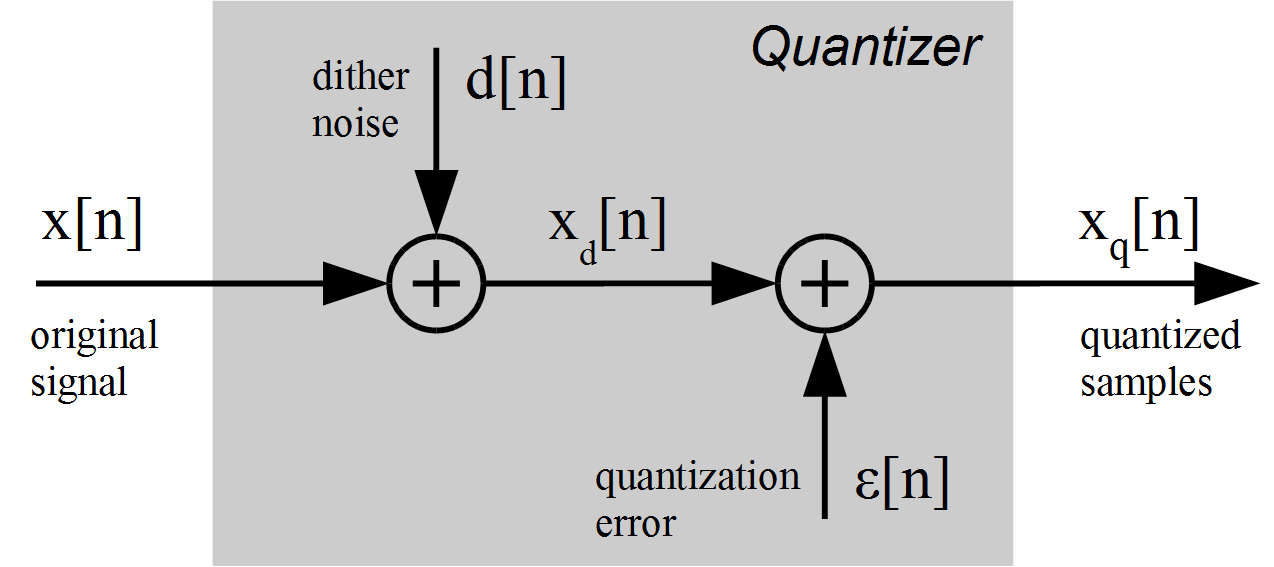
\includegraphics[width=.5\textwidth]{../fig/dithering}
\end{center}